% ============================================================
% Question Bank: ch06-07 Transformations on the Coordinate Plane
% Topic Title: Transformations on the Coordinate Plane
% CCSS: Supplementary (IN, VA)
% Questions: 30 (18 MC + 7 SA + 5 Graphical)
% ============================================================

% --- Multiple Choice Questions (18) ---

\begin{practiceQuestion}{6-7-q01}{mc}
\begin{questionText}
Point $A(3, 5)$ is translated right $4$ and down $2$. What are the coordinates of $A'$?
\end{questionText}
\choiceA{$(7, 7)$}
\choiceB{$(7, 3)$}
\choiceC{$(-1, 7)$}
\choiceD{$(-1, 3)$}
\correctAnswer{B}
\explanation{Right $4$: $3 + 4 = 7$. Down $2$: $5 - 2 = 3$. So $A'(7, 3)$.}
\end{practiceQuestion}

\begin{practiceQuestion}{6-7-q02}{mc}
\begin{questionText}
Point $B(-2, 4)$ is reflected over the $x$-axis. What are the coordinates of $B'$?
\end{questionText}
\choiceA{$(-2, -4)$}
\choiceB{$(2, 4)$}
\choiceC{$(2, -4)$}
\choiceD{$(-2, 4)$}
\correctAnswer{A}
\explanation{Reflection over the $x$-axis: keep $x$, negate $y$. $(-2, 4) \to (-2, -4)$.}
\end{practiceQuestion}

\begin{practiceQuestion}{6-7-q03}{mc}
\begin{questionText}
Point $C(5, -3)$ is reflected over the $y$-axis. What are the coordinates of $C'$?
\end{questionText}
\choiceA{$(5, 3)$}
\choiceB{$(-5, -3)$}
\choiceC{$(-5, 3)$}
\choiceD{$(3, -5)$}
\correctAnswer{B}
\explanation{Reflection over the $y$-axis: negate $x$, keep $y$. $(5, -3) \to (-5, -3)$.}
\end{practiceQuestion}

\begin{practiceQuestion}{6-7-q04}{mc}
\begin{questionText}
Point $D(2, 6)$ is rotated $90°$ clockwise about the origin. What are the coordinates of $D'$?
\end{questionText}
\choiceA{$(-6, 2)$}
\choiceB{$(6, -2)$}
\choiceC{$(-2, -6)$}
\choiceD{$(6, 2)$}
\correctAnswer{B}
\explanation{$90°$ clockwise: $(x, y) \to (y, -x)$. $(2, 6) \to (6, -2)$.}
\end{practiceQuestion}

\begin{practiceQuestion}{6-7-q05}{mc}
\begin{questionText}
Which transformation changes the position of a figure without changing its size, shape, or orientation?
\end{questionText}
\choiceA{Reflection}
\choiceB{Rotation}
\choiceC{Translation}
\choiceD{Dilation}
\correctAnswer{C}
\explanation{A translation (slide) moves every point the same distance and direction. The figure keeps its size, shape, and orientation.}
\end{practiceQuestion}

\begin{practiceQuestion}{6-7-q06}{mc}
\begin{questionText}
Point $E(-4, -1)$ is translated left $3$ and up $5$. What are the coordinates of $E'$?
\end{questionText}
\choiceA{$(-7, 4)$}
\choiceB{$(-1, -6)$}
\choiceC{$(-1, 4)$}
\choiceD{$(-7, -6)$}
\correctAnswer{A}
\explanation{Left $3$: $-4 - 3 = -7$. Up $5$: $-1 + 5 = 4$. So $E'(-7, 4)$.}
\end{practiceQuestion}

\begin{practiceQuestion}{6-7-q07}{mc}
\begin{questionText}
Point $F(0, -5)$ is reflected over the $x$-axis. What are the coordinates of $F'$?
\end{questionText}
\choiceA{$(0, 5)$}
\choiceB{$(0, -5)$}
\choiceC{$(5, 0)$}
\choiceD{$(-5, 0)$}
\correctAnswer{A}
\explanation{Over the $x$-axis: keep $x$, negate $y$. $(0, -5) \to (0, 5)$.}
\end{practiceQuestion}

\begin{practiceQuestion}{6-7-q08}{mc}
\begin{questionText}
Point $G(1, 4)$ is rotated $90°$ clockwise about the origin. Then the result is reflected over the $x$-axis. What are the final coordinates?
\end{questionText}
\choiceA{$(4, 1)$}
\choiceB{$(-4, -1)$}
\choiceC{$(4, -1)$}
\choiceD{$(-4, 1)$}
\correctAnswer{A}
\explanation{$90°$ clockwise: $(1, 4) \to (4, -1)$. Reflect over $x$-axis: $(4, -1) \to (4, 1)$. Final: $(4, 1)$.}
\end{practiceQuestion}

\begin{practiceQuestion}{6-7-q09}{mc}
\begin{questionText}
A triangle has vertices $P(1, 2)$, $Q(4, 2)$, and $R(4, 6)$. After a translation, $P' = (3, 0)$. What translation was applied?
\end{questionText}
\choiceA{Right $2$, down $2$}
\choiceB{Left $2$, up $2$}
\choiceC{Right $2$, up $2$}
\choiceD{Left $2$, down $2$}
\correctAnswer{A}
\explanation{From $P(1, 2)$ to $P'(3, 0)$: $x$ changed by $+2$ (right $2$) and $y$ changed by $-2$ (down $2$).}
\end{practiceQuestion}

\begin{practiceQuestion}{6-7-q10}{mc}
\begin{questionText}
Point $H(-3, 7)$ is reflected over the $y$-axis. What are the coordinates of $H'$?
\end{questionText}
\choiceA{$(-3, -7)$}
\choiceB{$(3, 7)$}
\choiceC{$(3, -7)$}
\choiceD{$(7, -3)$}
\correctAnswer{B}
\explanation{Over the $y$-axis: negate $x$, keep $y$. $(-3, 7) \to (3, 7)$.}
\end{practiceQuestion}

\begin{practiceQuestion}{6-7-q11}{mc}
\begin{questionText}
Which of the following is true about all three rigid transformations (translation, reflection, rotation)?
\end{questionText}
\choiceA{They all change the size of the figure}
\choiceB{They all preserve the size and shape of the figure}
\choiceC{They all keep the figure's orientation the same}
\choiceD{They all move the figure to the right}
\correctAnswer{B}
\explanation{Translations, reflections, and rotations are all rigid motions — they preserve size and shape. Reflections reverse orientation, and rotations change direction, but all keep the figure congruent.}
\end{practiceQuestion}

\begin{practiceQuestion}{6-7-q12}{mc}
\begin{questionText}
Point $J(6, -2)$ is rotated $90°$ clockwise about the origin. What are the coordinates of $J'$?
\end{questionText}
\choiceA{$(2, 6)$}
\choiceB{$(-2, -6)$}
\choiceC{$(-6, 2)$}
\choiceD{$(-2, 6)$}
\correctAnswer{B}
\explanation{$90°$ clockwise: $(x, y) \to (y, -x)$. $(6, -2) \to (-2, -6)$.}
\end{practiceQuestion}

\begin{practiceQuestion}{6-7-q13}{mc}
\begin{questionText}
After reflecting point $K$ over the $x$-axis, the image is $K'(4, -3)$. What were the original coordinates of $K$?
\end{questionText}
\choiceA{$(4, 3)$}
\choiceB{$(-4, -3)$}
\choiceC{$(-4, 3)$}
\choiceD{$(4, -3)$}
\correctAnswer{A}
\explanation{Reflection over the $x$-axis negates $y$. To reverse: $K'(4, -3) \to K(4, 3)$.}
\end{practiceQuestion}

\begin{practiceQuestion}{6-7-q14}{mc}
\begin{questionText}
A rectangle has vertices $A(1, 1)$, $B(5, 1)$, $C(5, 3)$, $D(1, 3)$. It is translated left $3$ and up $4$. What are the coordinates of $C'$?
\end{questionText}
\choiceA{$(2, 7)$}
\choiceB{$(8, 7)$}
\choiceC{$(2, -1)$}
\choiceD{$(8, -1)$}
\correctAnswer{A}
\explanation{$C(5, 3)$: left $3$ means $5 - 3 = 2$, up $4$ means $3 + 4 = 7$. So $C'(2, 7)$.}
\end{practiceQuestion}

\begin{practiceQuestion}{6-7-q15}{mc}
\begin{questionText}
Point $L(-1, -4)$ is reflected over the $y$-axis and then translated up $3$. What are the final coordinates?
\end{questionText}
\choiceA{$(1, -1)$}
\choiceB{$(-1, -1)$}
\choiceC{$(1, -7)$}
\choiceD{$(-1, 1)$}
\correctAnswer{A}
\explanation{Reflect over $y$-axis: $(-1, -4) \to (1, -4)$. Translate up $3$: $(1, -4 + 3) = (1, -1)$.}
\end{practiceQuestion}

\begin{practiceQuestion}{6-7-q16}{mc}
\begin{questionText}
A point is at the origin $(0, 0)$. It is rotated $90°$ clockwise. Where does it end up?
\end{questionText}
\choiceA{$(0, 0)$}
\choiceB{$(1, 0)$}
\choiceC{$(0, -1)$}
\choiceD{$(0, 1)$}
\correctAnswer{A}
\explanation{Rotating the origin about itself keeps it at $(0, 0)$. Any rotation of a point about itself results in no change.}
\end{practiceQuestion}

\begin{practiceQuestion}{6-7-q17}{mc}
\begin{questionText}
Point $M(3, -5)$ is reflected over the $x$-axis and then over the $y$-axis. What are the final coordinates?
\end{questionText}
\choiceA{$(3, 5)$}
\choiceB{$(-3, -5)$}
\choiceC{$(-3, 5)$}
\choiceD{$(3, -5)$}
\correctAnswer{C}
\explanation{Over $x$-axis: $(3, -5) \to (3, 5)$. Over $y$-axis: $(3, 5) \to (-3, 5)$.}
\end{practiceQuestion}

\begin{practiceQuestion}{6-7-q18}{mc}
\begin{questionText}
A figure is translated so that point $(2, 7)$ moves to $(2, 3)$. What translation was applied?
\end{questionText}
\choiceA{Up $4$}
\choiceB{Down $4$}
\choiceC{Left $4$}
\choiceD{Right $4$}
\correctAnswer{B}
\explanation{The $x$-coordinate stayed the same. The $y$-coordinate went from $7$ to $3$, a change of $-4$. That is down $4$.}
\end{practiceQuestion}

% --- Short Answer Questions (7) ---

\begin{practiceQuestion}{6-7-q19}{sa}
\begin{questionText}
Translate point $N(5, -2)$ left $6$ and up $3$. What are the coordinates of $N'$?
\end{questionText}
\correctAnswer{$N'(-1, 1)$}
\explanation{Left $6$: $5 - 6 = -1$. Up $3$: $-2 + 3 = 1$. So $N'(-1, 1)$.}
\end{practiceQuestion}

\begin{practiceQuestion}{6-7-q20}{sa}
\begin{questionText}
Reflect point $P(-6, 2)$ over the $x$-axis. What are the coordinates of $P'$?
\end{questionText}
\correctAnswer{$P'(-6, -2)$}
\explanation{Over the $x$-axis: keep $x$, negate $y$. $(-6, 2) \to (-6, -2)$.}
\end{practiceQuestion}

\begin{practiceQuestion}{6-7-q21}{sa}
\begin{questionText}
Rotate point $Q(4, -3)$ by $90°$ clockwise about the origin. What are the coordinates of $Q'$?
\end{questionText}
\correctAnswer{$Q'(-3, -4)$}
\explanation{$90°$ clockwise: $(x, y) \to (y, -x)$. $(4, -3) \to (-3, -4)$.}
\end{practiceQuestion}

\begin{practiceQuestion}{6-7-q22}{sa}
\begin{questionText}
A triangle has vertices $A(2, 1)$, $B(6, 1)$, and $C(6, 4)$. Reflect the triangle over the $y$-axis. List the new vertices.
\end{questionText}
\correctAnswer{$A'(-2, 1)$, $B'(-6, 1)$, $C'(-6, 4)$}
\explanation{Over the $y$-axis: negate $x$, keep $y$. $(2,1) \to (-2,1)$, $(6,1) \to (-6,1)$, $(6,4) \to (-6,4)$.}
\end{practiceQuestion}

\begin{practiceQuestion}{6-7-q23}{sa}
\begin{questionText}
Point $R$ is translated right $5$ and down $1$ to get $R'(3, 2)$. What were the original coordinates of $R$?
\end{questionText}
\correctAnswer{$R(-2, 3)$}
\explanation{Reverse the translation: left $5$ and up $1$. $x$: $3 - 5 = -2$. $y$: $2 + 1 = 3$. So $R(-2, 3)$.}
\end{practiceQuestion}

\begin{practiceQuestion}{6-7-q24}{sa}
\begin{questionText}
Point $S(-3, -5)$ is reflected over the $x$-axis, then translated right $4$. What are the final coordinates?
\end{questionText}
\correctAnswer{$(1, 5)$}
\explanation{Reflect over $x$-axis: $(-3, -5) \to (-3, 5)$. Translate right $4$: $(-3 + 4, 5) = (1, 5)$.}
\end{practiceQuestion}

\begin{practiceQuestion}{6-7-q25}{sa}
\begin{questionText}
What single transformation maps $(x, y)$ to $(-x, -y)$?
\end{questionText}
\correctAnswer{A $180°$ rotation about the origin}
\explanation{Negating both coordinates is equivalent to rotating $180°$ about the origin. It is also equivalent to reflecting over both axes.}
\end{practiceQuestion}

% --- Graphical Questions (3 GMC + 2 GSA) ---

\begin{practiceQuestion}{6-7-q26}{gmc}
\begin{questionText}
The graph shows triangle $ABC$ and its image $A'B'C'$. What transformation was performed?

\begin{center}
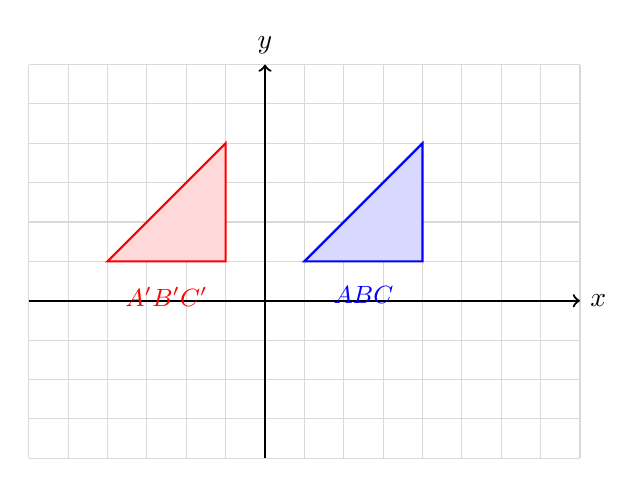
\begin{tikzpicture}[scale=0.5]
  \draw[step=1,gray!30,thin] (-6,-4) grid (8,6);
  \draw[thick,->] (-6,0) -- (8,0) node[right]{$x$};
  \draw[thick,->] (0,-4) -- (0,6) node[above]{$y$};
  % Original
  \draw[thick,blue,fill=blue!15] (1,1) -- (4,1) -- (4,4) -- cycle;
  \node[blue,below] at (2.5,0.6) {\small $ABC$};
  % Image
  \draw[thick,red,fill=red!15] (-4,1) -- (-1,1) -- (-1,4) -- cycle;
  \node[red,below] at (-2.5,0.6) {\small $A'B'C'$};
\end{tikzpicture}
\end{center}
\end{questionText}
\choiceA{Translation left $5$}
\choiceB{Reflection over the $y$-axis}
\choiceC{Rotation $90°$ clockwise}
\choiceD{Reflection over the $x$-axis}
\correctAnswer{B}
\explanation{Each point's $x$-coordinate is negated while $y$ stays the same: $(1,1) \to (-1,1)$, $(4,1) \to (-4,1)$, $(4,4) \to (-4,4)$. This is a reflection over the $y$-axis.}
\end{practiceQuestion}

\begin{practiceQuestion}{6-7-q27}{gmc}
\begin{questionText}
Point $T$ is shown on the coordinate plane. It is translated right $3$ and up $4$. Where is $T'$?

\begin{center}
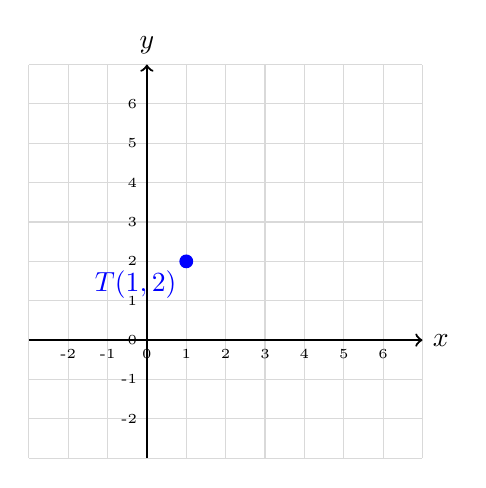
\begin{tikzpicture}[scale=0.5]
  \draw[step=1,gray!30,thin] (-3,-3) grid (7,7);
  \draw[thick,->] (-3,0) -- (7,0) node[right]{$x$};
  \draw[thick,->] (0,-3) -- (0,7) node[above]{$y$};
  \fill[blue] (1,2) circle (5pt);
  \node[below left,blue] at (1,2) {$T(1,2)$};
  \foreach \x in {-2,...,6} \node[below,font=\tiny] at (\x,0) {\x};
  \foreach \y in {-2,...,6} \node[left,font=\tiny] at (0,\y) {\y};
\end{tikzpicture}
\end{center}
\end{questionText}
\choiceA{$(4, 6)$}
\choiceB{$(4, -2)$}
\choiceC{$(-2, 6)$}
\choiceD{$(1, 6)$}
\correctAnswer{A}
\explanation{Right $3$: $1 + 3 = 4$. Up $4$: $2 + 4 = 6$. So $T'(4, 6)$.}
\end{practiceQuestion}

\begin{practiceQuestion}{6-7-q28}{gmc}
\begin{questionText}
The coordinate plane shows point $U$ and its image $U'$ after a reflection. Over which axis was $U$ reflected?

\begin{center}
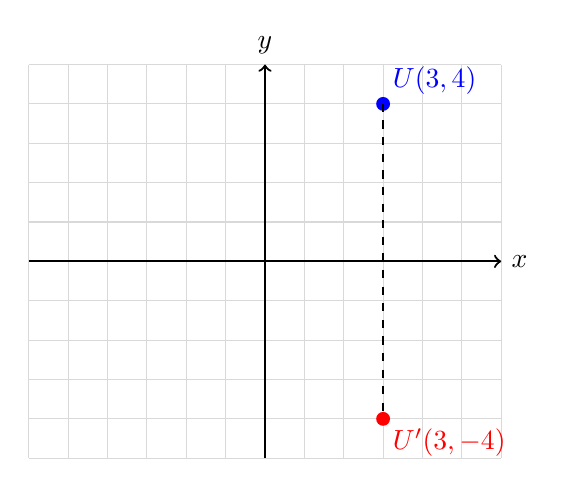
\begin{tikzpicture}[scale=0.5]
  \draw[step=1,gray!30,thin] (-6,-5) grid (6,5);
  \draw[thick,->] (-6,0) -- (6,0) node[right]{$x$};
  \draw[thick,->] (0,-5) -- (0,5) node[above]{$y$};
  \fill[blue] (3,4) circle (5pt);
  \node[above right,blue] at (3,4) {$U(3,4)$};
  \fill[red] (3,-4) circle (5pt);
  \node[below right,red] at (3,-4) {$U'(3,-4)$};
  \draw[dashed,thick] (3,4) -- (3,-4);
\end{tikzpicture}
\end{center}
\end{questionText}
\choiceA{The $x$-axis}
\choiceB{The $y$-axis}
\choiceC{The line $y = x$}
\choiceD{The line $x = 3$}
\correctAnswer{A}
\explanation{The $x$-coordinate stayed the same ($3$) and the $y$-coordinate changed sign ($4 \to -4$). This is a reflection over the $x$-axis.}
\end{practiceQuestion}

\begin{practiceQuestion}{6-7-q29}{gsa}
\begin{questionText}
The coordinate plane shows a rectangle with vertices $A(1, 1)$, $B(5, 1)$, $C(5, 3)$, $D(1, 3)$. Reflect the rectangle over the $x$-axis and list the new vertices.

\begin{center}
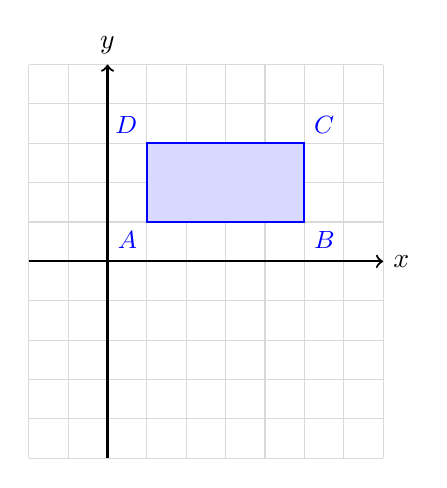
\begin{tikzpicture}[scale=0.5]
  \draw[step=1,gray!30,thin] (-2,-5) grid (7,5);
  \draw[thick,->] (-2,0) -- (7,0) node[right]{$x$};
  \draw[thick,->] (0,-5) -- (0,5) node[above]{$y$};
  \draw[thick,blue,fill=blue!15] (1,1) -- (5,1) -- (5,3) -- (1,3) -- cycle;
  \node[above left,blue,font=\small] at (1,3) {$D$};
  \node[above right,blue,font=\small] at (5,3) {$C$};
  \node[below left,blue,font=\small] at (1,1) {$A$};
  \node[below right,blue,font=\small] at (5,1) {$B$};
\end{tikzpicture}
\end{center}
\end{questionText}
\correctAnswer{$A'(1, -1)$, $B'(5, -1)$, $C'(5, -3)$, $D'(1, -3)$}
\explanation{Over the $x$-axis: keep $x$, negate $y$. $(1,1) \to (1,-1)$, $(5,1) \to (5,-1)$, $(5,3) \to (5,-3)$, $(1,3) \to (1,-3)$.}
\end{practiceQuestion}

\begin{practiceQuestion}{6-7-q30}{gsa}
\begin{questionText}
The graph shows triangle $PQR$ with $P(2, 3)$, $Q(5, 3)$, and $R(5, 7)$. Rotate the triangle $90°$ clockwise about the origin. List the new vertices.

\begin{center}
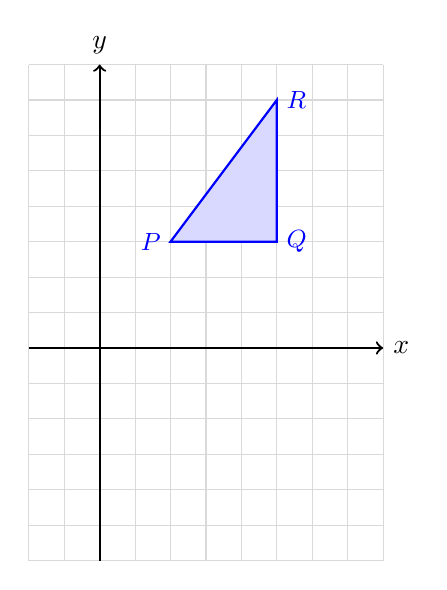
\begin{tikzpicture}[scale=0.45]
  \draw[step=1,gray!30,thin] (-2,-6) grid (8,8);
  \draw[thick,->] (-2,0) -- (8,0) node[right]{$x$};
  \draw[thick,->] (0,-6) -- (0,8) node[above]{$y$};
  \draw[thick,blue,fill=blue!15] (2,3) -- (5,3) -- (5,7) -- cycle;
  \node[left,blue,font=\small] at (2,3) {$P$};
  \node[right,blue,font=\small] at (5,3) {$Q$};
  \node[right,blue,font=\small] at (5,7) {$R$};
\end{tikzpicture}
\end{center}
\end{questionText}
\correctAnswer{$P'(3, -2)$, $Q'(3, -5)$, $R'(7, -5)$}
\explanation{$90°$ clockwise: $(x, y) \to (y, -x)$. $P(2,3) \to (3,-2)$, $Q(5,3) \to (3,-5)$, $R(5,7) \to (7,-5)$.}
\end{practiceQuestion}
